Based on the signal regions defined in Section~\ref{sec:strategy.sr}, 
it is useful to evaluate the signal acceptance of the analysis using 
parton level MC simulation (truth study). The acceptance encodes all the 
kinematic cuts applied on the signal as well as the branching ratios of 
all the decay particles. This information 
will help us understand the sensitivity reach of the analysis and also allow 
theorists to use this information when comparing the simplified model 
results to their models. 
The signal acceptance is shown in Figure~\ref{fig:strategy.accRpc2L0bH} with 
the rest of the 
signal regions shown in Appendix~\ref{app:aux.AccEff}.
Table~\ref{tab:strategy.cut} shows an example of a detailed cut-flow 
for weighted signal MC events illustrating the impact of cuts from the 
Rpc2L0bH signal region on a signal model. More tables are shown in 
Appendix~\ref{app:aux.SRcut}. 
\begin{figure}[htb!]
\centering
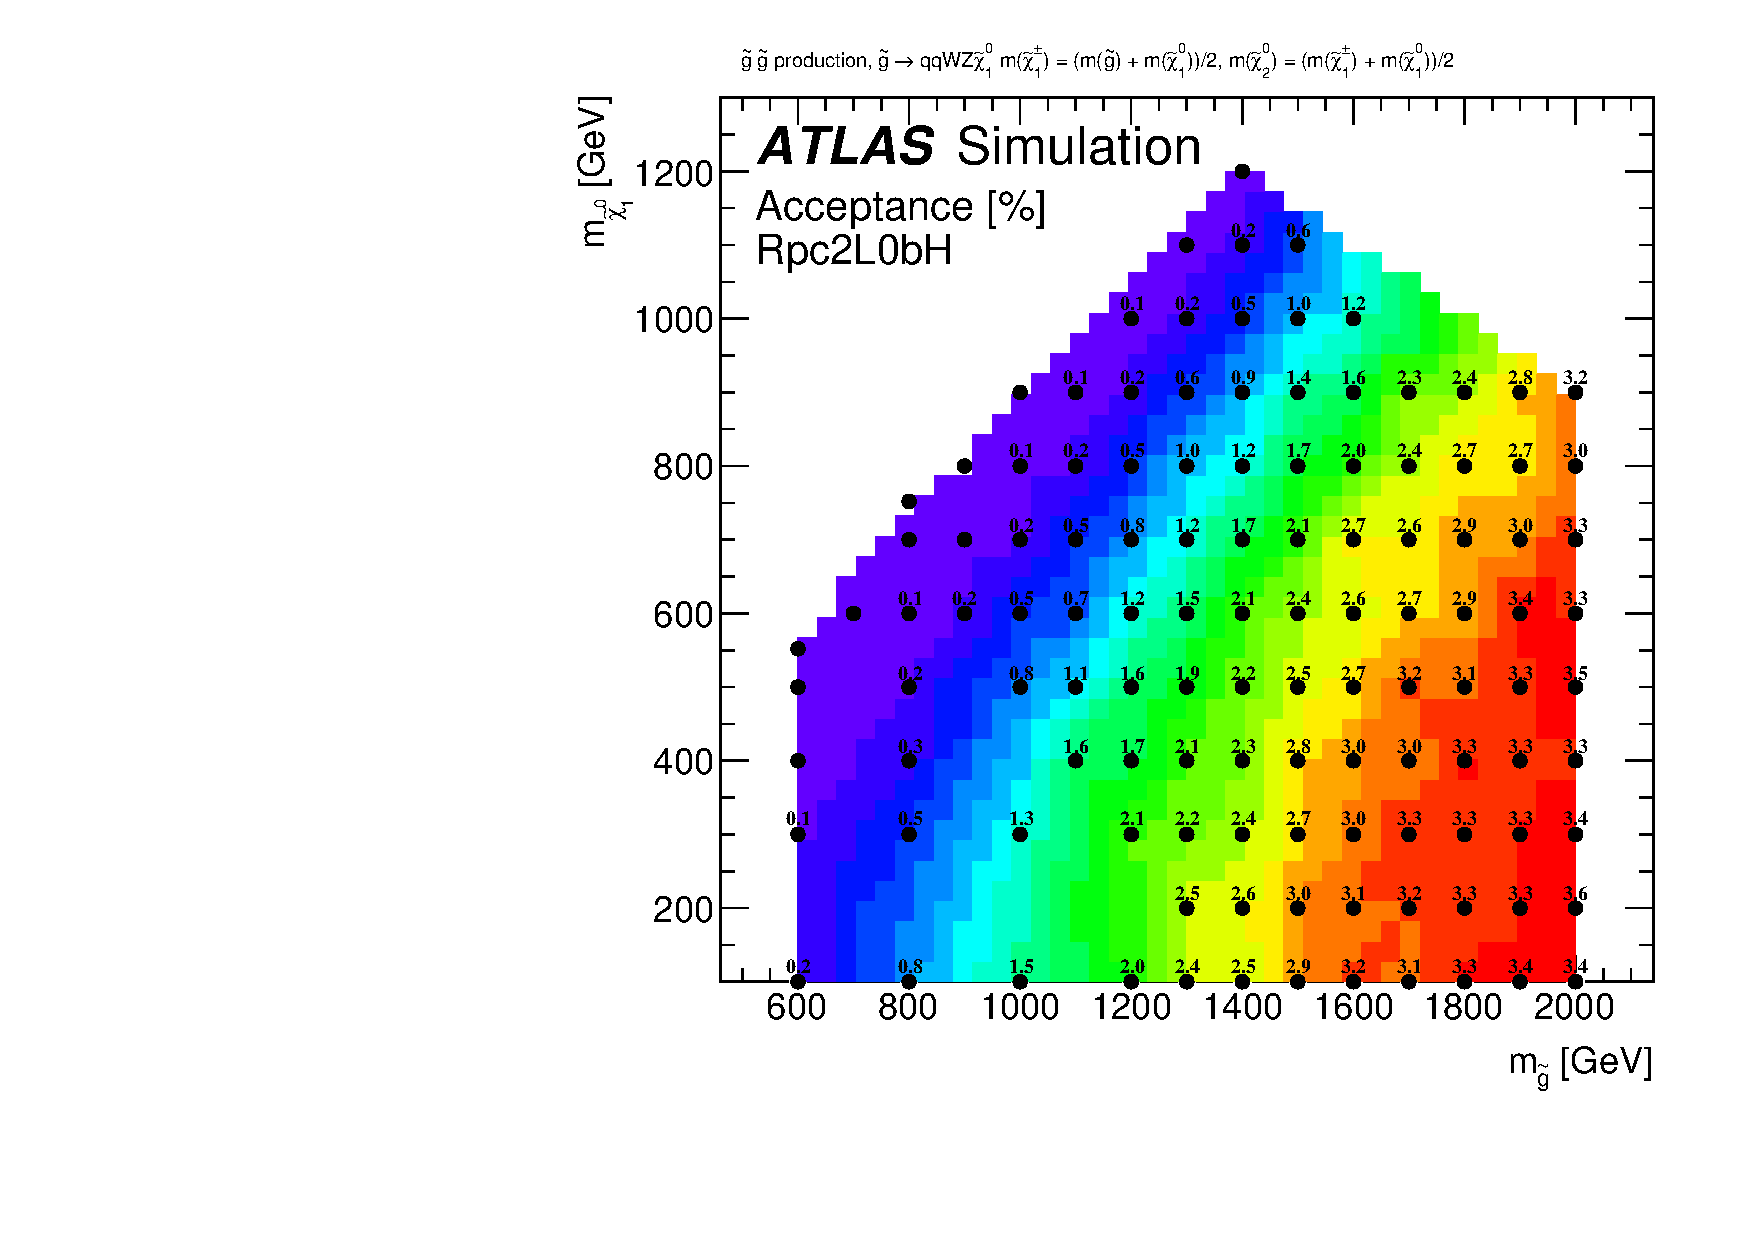
\includegraphics[width=\textwidth]{EffAcc/acceptance_2StepRpc2L0bH}
\caption{Signal acceptance for simplified models of $\gluino\gluino$ production with $\gluino\to q\bar q^{'}WZ\ninoone$ decays, 
in the signal regions Rpc2L0bH.}
\label{fig:strategy.accRpc2L0bH}
\end{figure}
\begin{table}[ht]\centering\def\arraystretch{1.2}\begin{tabular}{|l|c|}\hline
   \multicolumn{2}{|l|}{Rpc2L0bH,\quad$\gluino\gluino$ production,\quad$\gluino\to q\bar q^{'}WZ\ninoone$}\\
   \multicolumn{2}{|l|}{$m_{\gluino}=1.6 \TeV$, $(m_{\chargino} - 750) = (m_{\tilde\chi_2^0} - 375) = m_{\ninoone}=100 \GeV$}\\\hline
   MC events generated  & 20000 \\\hline
   Expected for 36.1 \ifb  & $2.9\times 10^2$ \\
   $\geq 2$ SS leptons ($\pt>20 \GeV$)  & $12.8 \pm 0.5$ \\
   Trigger  & $12.5 \pm 0.5$ \\
   no $b$-jet ($\pt>20 \GeV$)  & $8.5 \pm 0.4$ \\
   $\ge 6$ jets ($\pt>40 \GeV$)  & $7.12 \pm 0.35$ \\
   $\met>250 \GeV$  & $5.13 \pm 0.29$ \\
   $\meff>0.9 \TeV$  & $5.13 \pm 0.29$ \\
\hline\end{tabular}
\caption{Number of signal events at different stages of the Rpc2L0bH signal region selection. 
Only statistical uncertainties are shown.}
\label{tab:strategy.cut}\end{table}

Another quantity of interest, to experimentalists in particular, is the detector
 efficiency that entails the reconstruction and identification efficiencies 
of the different particles used in the analysis. The efficiency $\epsilon$ 
can be obtained from the relation 
\begin{equation}
S = L_\text{int}\cdot\sigma_{\text{prod}}\cdot A\cdot\epsilon, 
\end{equation}
where $S$ is the expected number of signal events, $\sigma_{\text{prod}}$ is the 
production cross section of the signal process, $L_\text{int}$ is the integrated 
luminosity, and $A$ is the acceptance. 
Figure~\ref{fig:strategy.effRpc2L0bH} shows the efficiency map for one of the signal models 
with the rest of the signal models shown in Appendix~\ref{app:aux.AccEff}.
\begin{figure}[htb!]
\centering
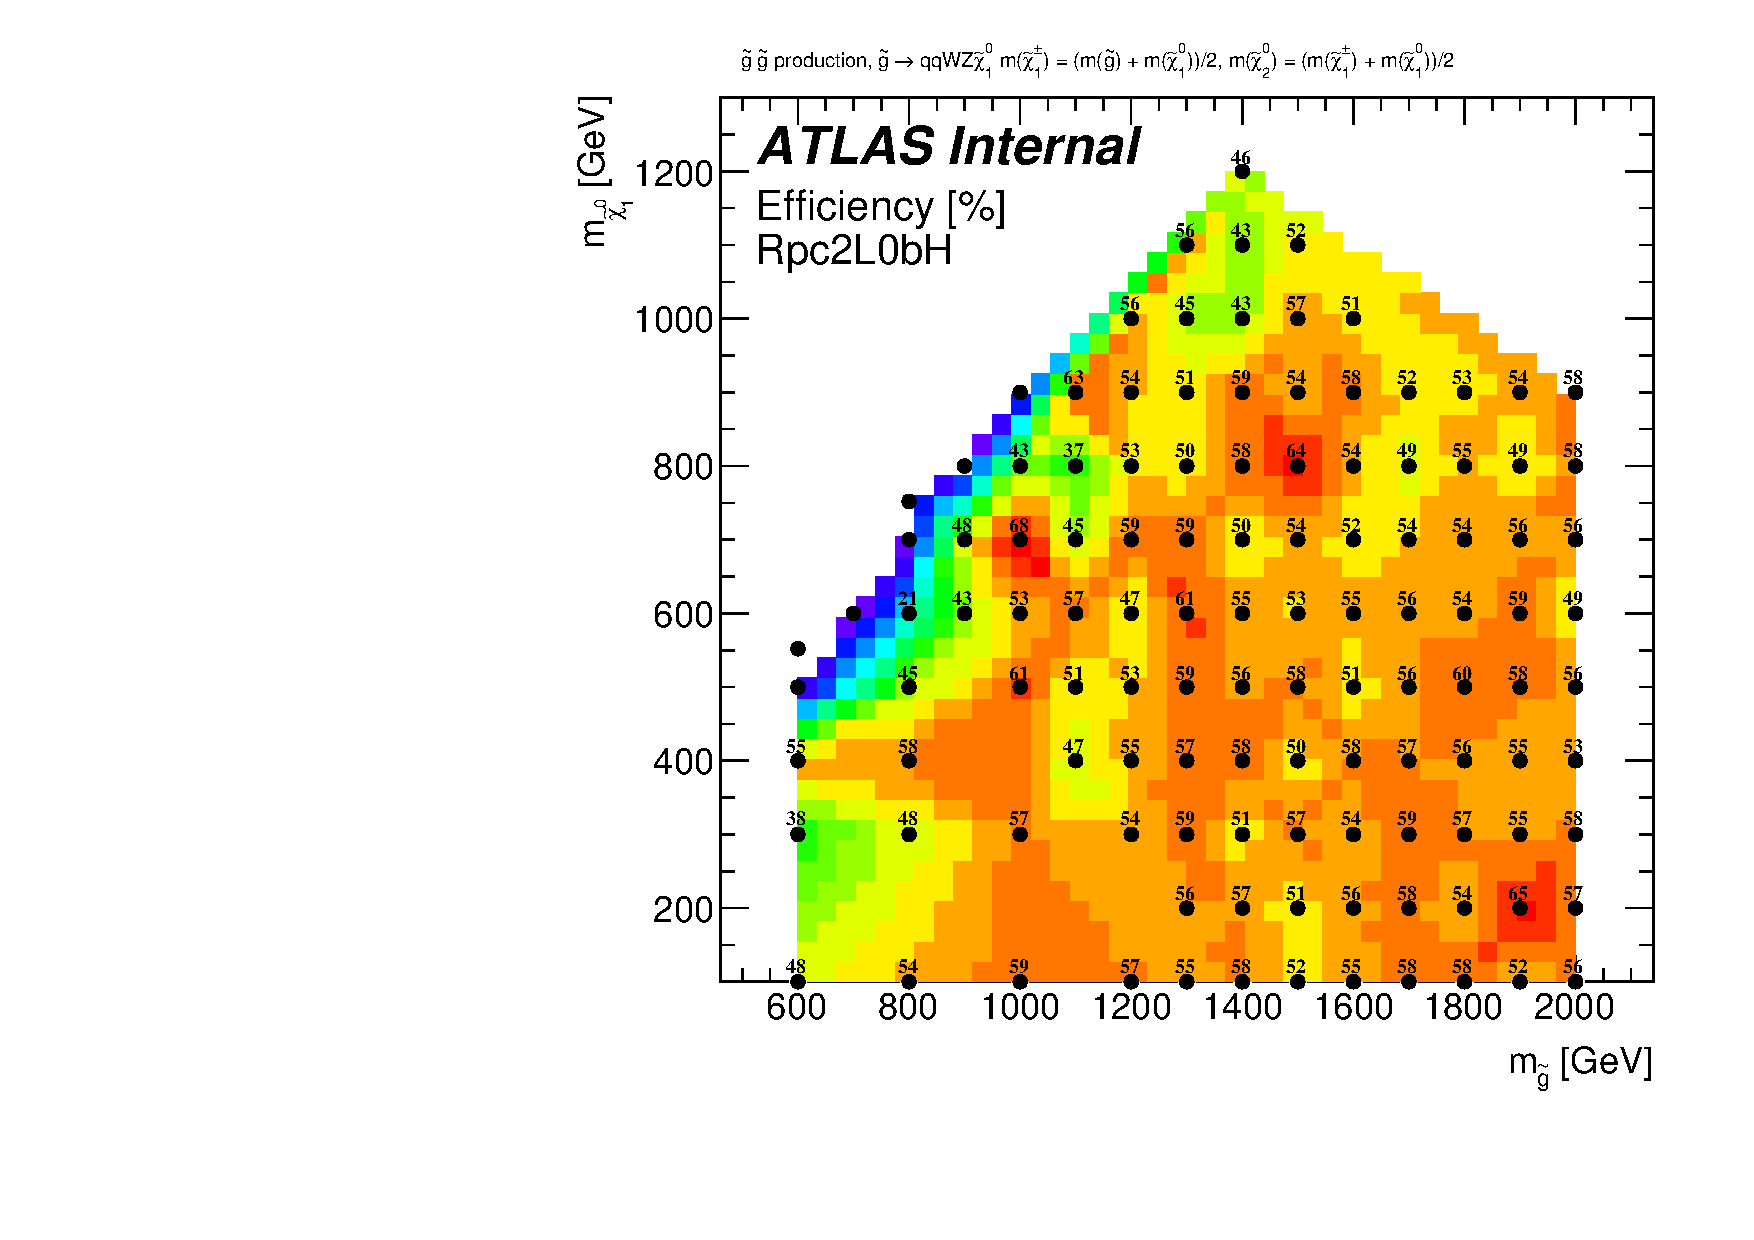
\includegraphics[width=\textwidth]{EffAcc/efficiency_2StepRpc2L0bH}
\caption{Signal reconstruction efficiency 
for simplified models of $\gluino\gluino$ production with $\gluino\to q\bar q^{'}WZ\ninoone$ decays, 
in the signal regions Rpc2L0bH.}
\label{fig:strategy.effRpc2L0bH}
\end{figure}
